% Sturm.tex
% Copyright (c) Sergey Strukov. All rights reserved. This is a public document. You can freely distribute and use it, providing the authorship and the copyright note is unchanged.

\input ../SSCommon.tex

\begin{document}
\selectlanguage{russian}
    
\SScover
    
\SStitle{Теорема Штурма}

Теорема Штурма --- красивая элементарная теорема школьного уровня. Она позволяет найти число корней данного полинома с вещественными коэффициентами на заданном интервале.
С её помощью можно локализовать корни вещественных полиномов и находить хорошие приближения к ним.

\vspace

\SSbullet 

\begin{tikzpicture}
    \draw[thick,->] (0,-2) -- (0,2) node[anchor=north west] {\(y\)};
    \draw[thick,->] (-2,0) -- (2,0) node[anchor=north west] {\(x\)};
    \draw (1,1) node[anchor=south west] {\(0\)};
    \draw (1,-1) node[anchor=north west] {\(1\)};
    \draw (-1,1) node[anchor=south east] {\(1\)};
    \draw (-1,-1) node[anchor=north east] {\(0\)};
\end{tikzpicture}

\SSsect[def] Функция \( \sigma: \xR^* \times \xR^* \rightarrow \{0,1\} \) определена как
\[ \sigma(x,y) := 
   \begin{cases} 
       1, & sign(x) = sign(y) \\ 
       0, & sign(x) \neq sign(y)
   \end{cases} 
\]

\SSsect \( \sigma(x,y) = \sigma(y,x) \)

\SSsect \( \sigma(-x,y) = 1 - \sigma(x,y) \)

\SSsect[def] \( \sigma(x_1,\dots,x_n) \) , \( x_1,\dots,x_n \in \xR^* \) , \( n \geqslant 1 \)
\[ \sigma(x_1,\dots,x_n) := \sum_{k=1}^{n-1} \sigma(x_k,x_{k+1})
\]
--- число перемен знака (Ч.П.З.)

\SSsect Индуктивно,
\begin{itemize}[label=]
\item \( \sigma(x_1) = 0 \) ,
\item \( \sigma(x_1,\dots,x_n) = \sigma(x_1,x_2) + \sigma(x_2,\dots,x_n) \) , \( n \geqslant 2 \) .
\end{itemize}

\vspace

\SSbullet

В этом пункте \( f,g \in \xR[T] \) .

\SSsect Пусть \( f \) и \( g \) не имеют общих вещественных корней. 
Пусть \( a,b \in \xR \) , \( a < b \) .

\SSsect Пусть \( a,b \) --- не корни \( f \) или \( g \) .
Т.е. \( f(a),g(a),f(b),g(b) \in \xR^* \) .

\SSsect[def] Определим \( \varphi(t) := \sigma(f(t),g(t)) \) , \( t \in \xR \) .
Тогда \( \varphi \) определена вне (конечного) множества корней \( f \) или \( g \) ,
например, в \( a \) и \( b \) .

\SSsect Функция \( \varphi(t) \) локально постоянна. Это вытекает из непрерывности \( f(t) \) ,
\( g(t) \) и локального постоянcтва \( \sigma(x,y) \) .

\vspace
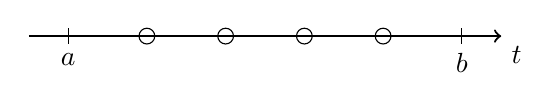
\begin{tikzpicture}
\draw[thick,->] (0,0) -- (6,0) node[anchor=north west] {\(t\)};    
\draw (0.5,0.1) -- (0.5,-0.1) node[anchor=north] {\(a\)};
\draw (5.5,0.1) -- (5.5,-0.1) node[anchor=north] {\(b\)};
\draw[] (1.5,0) circle [radius=0.1];
\draw[] (2.5,0) circle [radius=0.1];
\draw[] (3.5,0) circle [radius=0.1];
\draw[] (4.5,0) circle [radius=0.1];
\end{tikzpicture}


\SSsect[def] Определим \( \delta(t) := \varphi(t+0) - \varphi(t-0) \in \{-1,0,1\} \) --- 
функция скачков \( \varphi \) .

\SSsect \( \delta(t) = 0 \) вне корней \( f \) или \( g \) .

\SSsect[!!] Главная теорема:
\[ \varphi(b) - \varphi(a) = \sum_{ a<t<b \enspace \delta(t) \neq 0 } \delta(t) \]

\SSsect[def] Определим символ
\[ \left( \frac{f}{g} \right)^b_a := \sum_{ a<t<b \enspace g(t)=0 } \delta(t) \]

\SSsect \( \varphi \) и \( \delta \) для пар \( (f,g) \) и \( (g,f) \) одинаковы.

\SSsect[!!] Закон взаимности:
\[ \left( \frac{f}{g} \right)^b_a + \left( \frac{g}{f} \right)^b_a = \varphi(b)-\varphi(a) \]

\SSsect Если заменить \( f \) на \( -f \) , то \( \varphi \) превратиться в \( 1-\varphi \) , а \( \delta \) в \( -\delta \) .

\SSsect[!] Нечётность:
\[ \left( \frac{-f}{g} \right)^b_a = - \left( \frac{f}{g} \right)^b_a \]

\SSsect[!] Модулярность. Если заменить \( f \) на полином \( h \in \xR[T] \) , такой, что
\( g(t) = 0 \Rightarrow h(t) = f(t) \) , то значения \( \delta(t) \) не изменяться в точках
\( \{ t \in \xR : g(t) = 0 \} \) . Поэтому
\[ \left( \frac{h}{g} \right)^b_a = \left( \frac{f}{g} \right)^b_a \]
В частности, это верно, если \( h=f-qg \) . Для доказательства см. картинку:
\vspace
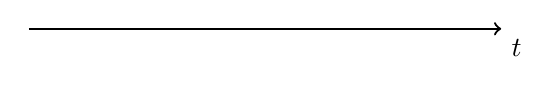
\begin{tikzpicture}
\draw[thick,->] (0,0) -- (6,0) node[anchor=north west] {\(t\)};    
\end{tikzpicture}

\vspace

\SSbullet

\SSbullet


\end{document}

